\PassOptionsToPackage{table,xcdraw,dvipsnames}{xcolor}

% ---------------------------------------------------------------------------
% Author guideline and sample document for EG publication using LaTeX2e input
% D.Fellner, v1.22, Jan 22, 2024

\documentclass{egpubl}
\usepackage{pgv2024}
 
% --- for  Annual CONFERENCE
% \ConferenceSubmission   % uncomment for Conference submission
% \ConferencePaper        % uncomment for (final) Conference Paper
% \STAR                   % uncomment for STAR contribution
% \Tutorial               % uncomment for Tutorial contribution
% \ShortPresentation      % uncomment for (final) Short Conference Presentation
% \Areas                  % uncomment for Areas contribution
% \Education              % uncomment for Education contribution
% \Poster                 % uncomment for Poster contribution
% \DC                     % uncomment for Doctoral Consortium
%
% --- for  CGF Journal
% \JournalSubmission    % uncomment for submission to Computer Graphics Forum
% \JournalPaper         % uncomment for final version of Journal Paper
%
% --- for  CGF Journal: special issue
% \SpecialIssueSubmission    % uncomment for submission to , special issue
% \SpecialIssuePaper         % uncomment for final version of Computer Graphics Forum, special issue
%                          % EuroVis, SGP, Rendering, PG
% --- for  EG Workshop Proceedings
% \WsSubmission      % uncomment for submission to EG Workshop
\WsPaper           % uncomment for final version of EG Workshop contribution
% \WsSubmissionJoint % for joint events, for example ICAT-EGVE
% \WsPaperJoint      % for joint events, for example ICAT-EGVE
% \WsPaperJointdemo         % uncomment for final version of EG Workshop contribution
% \WsPaperJointposter         % uncomment for final version of EG Workshop contribution 
% \WsPoster          % uncomment for Poster contribution
% \WsShortPaper      % uncomment for Short Paper contribution
% \Expressive        % for SBIM, CAe, NPAR
% \DigitalHeritagePaper
% \PaperL2P          % for events EG only asks for License to Publish

% --- for EuroVis 
% for full papers use \SpecialIssuePaper
% \STAREurovis   % for EuroVis additional material 
% \EuroVisPoster % for EuroVis additional material 
% \EuroVisShort  % for EuroVis additional material
% \MedicalPrize  % uncomment for Medical Prize (Dirk Bartz) contribution, since 2021 part of EuroVis
% \EuroVisEducation              % uncomment for Education contribution

% Licences: for CGF Journal (EG conf. full papers and STARs, EuroVis conf. full papers and STARs, SR, SGP, PG)
% please choose the correct license
%\CGFStandardLicense
%\CGFccby
%\CGFccbync
%\CGFccbyncnd

% !! *please* don't change anything above
% !! unless you REALLY know what you are doing
% ------------------------------------------------------------------------
\usepackage[T1]{fontenc}
\usepackage{dfadobe}  

\usepackage{cite}  % comment out for biblatex with backend=biber
% ---------------------------
%\biberVersion
\BibtexOrBiblatex
%\usepackage[backend=biber,bibstyle=EG,citestyle=alphabetic,backref=true]{biblatex} 
%\addbibresource{egbibsample.bib}
% ---------------------------  
\electronicVersion
\PrintedOrElectronic
% for including postscript figures
% mind: package option 'draft' will replace PS figure by a filename within a frame
\ifpdf \usepackage[pdftex]{graphicx} \pdfcompresslevel=9
\else \usepackage[dvips]{graphicx} \fi

\usepackage{egweblnk} 
\usepackage{microtype}                 % use micro-typography (slightly more compact, better to read)
\PassOptionsToPackage{warn}{textcomp}  % to address font issues with \textrightarrow
\usepackage{textcomp}                  % use better special symbols
\usepackage{mathptmx}                  % use matching math font
\usepackage{amsmath}
\usepackage{amstext}
\usepackage{amssymb}
\usepackage{times}                     % we use Times as the main font
\renewcommand*\ttdefault{txtt}         % a nicer typewriter font
\usepackage{tabu}                      % only used for the table example
\usepackage{booktabs}                  % only used for the table example
\usepackage{algorithm}
\usepackage{algpseudocode}
\usepackage{caption}
\usepackage{enumitem}
\setlist[enumerate]{topsep=0pt}
\usepackage{float}
\usepackage{graphicx}
\usepackage{hyperref}
\usepackage{listings}
\usepackage{multirow}
\usepackage{stfloats}
\usepackage{subcaption}
\usepackage{tikz}
\usetikzlibrary{decorations.pathreplacing,calc}
% \usepackage{orcidlink}
\usepackage[normalem]{ulem}
\usepackage{wrapfig}
\usepackage[table]{xcolor}
\captionsetup{labelfont=bf,textfont=it}

% ---------------------------------------------------------------------
% EG author guidelines plus sample file for EG publication using LaTeX2e input
% D.Fellner, v2.04, Sep 19, 2023

\title{An Accelerated Clip Algorithm for Unstructured Meshes:\\ A Batch-Driven Approach}

%% This is how authors are specified in the conference style

% ---------------------------------------------------------------------
% EG author guidelines plus sample file for EG publication using LaTeX2e input
% D.Fellner, v2.04, Sep 19, 2023

% for anonymous conference submission please enter your SUBMISSION ID
% instead of the author's name (and leave the affiliation blank) !!
% for final version: please provide your *own* ORCID in the brackets following \orcid; see https://orcid.org/ for more details.
\author
[
S. Tsalikis 
\& W. Schroeder
\& D. Szafir
\& K. Moreland
]
{\parbox{\textwidth}{\centering
Spiros Tsalikis $^{1,2}$
% \thanks{e-mail: spiros.tsalikis@\{kitware.com,cs.unc.edu\}}
\orcid{0000-0001-5113-7195},
Will Schroeder $^{1}$
% \thanks{e-mail: will.schroeder@kitware.com}
\orcid{0000-0003-3815-9386},
Daniel Szafir $^{2}$
% \thanks{e-mail: daniel.szafir@cs.unc.edu}
\orcid{0000-0003-1848-7884}
and
Kenneth Moreland $^{3}$
% \thanks{e-mail: morelandkd@ornl.gov}
\orcid{0000-0002-7051-3288}
}
\\
% For Computer Graphics Forum: Please use the abbreviation of your first name.
{\parbox{\textwidth}{\centering
$^1$Scientific Computing, Kitware, Inc., USA\\
$^2$Department of Computer Science, University of North Carolina at Chapel Hill, USA\\
$^3$Oak Ridge National Laboratory, USA
}
}
}
% ------------------------------------------------------------------------

\newcommand*{\fix}[1]{\textcolor{red}{#1}}


%-------------------------------------------------------------------------
\begin{document}

% uncomment for using teaser
% \teaser{
%  
\includegraphics[width=0.9\linewidth]{eg_new}
%  \centering
%   \caption{New EG Logo}
% \label{fig:teaser}
%}

\maketitle
%-------------------------------------------------------------------------
%% Abstract section.
\begin{abstract}
The clip technique is a popular method for visualizing complex structures and phenomena within 3D unstructured meshes.
Meshes can be clipped by specifying a scalar isovalue to produce an output unstructured mesh with its external surface as the isovalue.
Similar to isocontouring, the clipping process relies on scalar data associated with the mesh points, including scalar data generated by implicit functions such as planes, boxes, and spheres, which facilitates the visualization of results interior to the grid.
In this paper, we introduce a novel batch-driven parallel algorithm based on a sequential clip algorithm designed for high-quality results in partial volume extraction. Our algorithm comprises five passes, each progressively processing data to generate the resulting clipped unstructured mesh. The novelty lies in the use of fixed-size batches of points and cells, which enable rapid workload trimming and parallel processing, leading to a significantly improved memory footprint and run-time performance compared to the original version.
On a 32-core CPU, the proposed batch-driven parallel algorithm demonstrates a run-time speed-up of up to 32.6x and a memory footprint reduction of up to 4.37x compared to the existing sequential algorithm.  The software is currently available under an open-source license in the VTK visualization system.

%-------------------------------------------------------------------------
%  ACM CCS 1998
%  (see https://www.acm.org/publications/computing-classification-system/1998)
% \begin{classification} % according to https://www.acm.org/publications/computing-classification-system/1998
% \CCScat{Computer Graphics}{I.3.3}{Picture/Image Generation}{Line and curve generation}
% \end{classification}
%-------------------------------------------------------------------------
%  ACM CCS 2012
% (see https://www.acm.org/publications/class-2012)
   
\begin{CCSXML}
<ccs2012>
<concept>
<concept_id>10010147.10010169.10010170.10010171</concept_id>
<concept_desc>Computing methodologies~Shared memory algorithms</concept_desc>
<concept_significance>500</concept_significance>
</concept>
<concept>
<concept_id>10010147.10010371.10010396.10010398</concept_id>
<concept_desc>Computing methodologies~Mesh geometry models</concept_desc>
<concept_significance>500</concept_significance>
</concept>
<concept>
<concept_id>10003752.10010061.10010063</concept_id>
<concept_desc>Theory of computation~Computational geometry</concept_desc>
<concept_significance>500</concept_significance>
</concept>
</ccs2012>
\end{CCSXML}

\ccsdesc[500]{Computing methodologies~Shared memory algorithms}
% \ccsdesc[500]{Computing methodologies~Mesh geometry models}
\ccsdesc[500]{Theory of computation~Computational geometry}
\printccsdesc   
\end{abstract}

%%%%%%%%%%%%%%%%%%%%%%%%%%%%%%%%%%%%%%%%%%%%%%%
% INTRODUCTION
%%%%%%%%%%%%%%%%%%%%%%%%%%%%%%%%%%%%%%%%%%%%%%%
\section{Introduction}

Current computing trends are driven by the increasing size of data and the evolution of parallel computing systems. However, many popular algorithms were originally designed for sequential computing models, which may reduce their effectiveness in modern applications. For example,  Marching cubes \cite{MC, MCSurvey}, a well-known isocontouring algorithm, widely employed in visualization software like VTK \cite{VTKBook}, ParaView \cite{ParaView}, and VisIt \cite{VisIt}, inherits sequential design patterns that adversely affect performance. These patterns include building data structures incrementally for inserting output points and cells, incremental memory allocations, and duplication of computational operations to produce intermediate results. These deficiencies prompted the recent development of Flying Edges \cite{FE}, a performant and scalable algorithm that addresses the computational shortcomings of Marching Cubes.

In this work, our goal is to accelerate the sequential clip algorithm introduced by Meredith et al. \cite{Clip}, which shares similar deficiencies with those found in Marching Cubes. This algorithm is designed with the primary goal of reconstructing material interfaces from volume fractions for visualization and analysis purposes. It is capable of processing both discrete and continuous data; however, this paper focuses solely on its continuous version due to its simplicity. Furthermore, it exhibits desirable quality across multiple accuracy metrics, generating smooth surfaces with minimal defects. Thanks to these noteworthy features, this clip algorithm is widely recognized as an important visualization technique for visually exploring complex unstructured meshes.

\textbf{Contributions}:
In this paper, inspired by the emergence of new parallel computing models, we introduce a high-performance batch-driven parallel clip algorithm optimized for unstructured meshes. Following the example set by Flying Edges, our proposed algorithm represents a redesign of Meredith's sequential clip algorithm, tailored to exploit modern multi-core hardware.
Our parallel multi-pass algorithm has the following novel contributions:
\begin{enumerate}
    \item Eliminates bottleneck functions, such as coincident point merging, and reduces incremental memory allocations.
    \item Minimizes memory accesses by reducing memory footprint, optimizing cache-friendly access, and avoiding unnecessary accesses.
    \item Utilizes fixed-size batches of points and cells, enabling rapid workload trimming and parallel processing.
    \item Significantly surpasses both Meredith's sequential algorithm and VTK-m's \cite{VTKm} parallel algorithm in terms of performance and memory footprint. Additionally, it demonstrates enchanced parallel efficiency compared to VTK-m's algorithm.
\end{enumerate}

\begin{figure}[h]
  \centering
  \includegraphics[width=\linewidth]{./Figures/JSM-Clip.png}
  \caption{An interior view of the external surface of the Japan Aerospace Exploration Agency (JAXA) Standard Model (JSM), from the 3rd AIAA CFD High-Lift Prediction Workshop \cite{JAXAModel}, that was clipped in half using a plane.}
  \label{fig:jaxa-model}
\end{figure}

In the following sections, we cover related work, define the problem, discuss Meredith's sequential clip algorithm, introduce our batch-driven parallel clip algorithm, evaluate performance and discuss the results, and conclude with future work.

%%%%%%%%%%%%%%%%%%%%%%%%%%%%%%%%%%%%%%%%%%%%%%%
% Related Work
%%%%%%%%%%%%%%%%%%%%%%%%%%%%%%%%%%%%%%%%%%%%%%%
\section{Related Work}
\label{sec:related-work}

Prior research has proposed several approaches for implementing a clip algorithm. All of these approaches share the common goal of removing portions of a mesh that are unimportant or interfere with visual inspection or data processing. As Figure \ref{fig:jaxa-model} illustrates, this may involve removing specific regions of the mesh in space or defining values of a field that should be removed.

Clipping algorithms are typically implemented by processing the cells of a mesh. For each input cell of a mesh, a clip algorithm computes a case index based on the scalar values of its defining points, akin to Marching Cubes, to access a case table. A case table indicates whether a cell produces nothing, the cell itself, or one or more new clipped cells. The output cells reference three types of points: input points, edge point intersections defined by two input points, and points located at the centroid of input cells.

The VTK library's \cite{VTK} first clip algorithm, which is still available today within the \texttt{vtkClipDataSet} class, has a single pass. During this pass, the algorithm fully extracts each input cell, computes the case index to access a case table, and generates output cells and points, incrementally. Notably, a point locator is employed to identify duplicate points before they are incrementally added. This algorithm exhibits three noteworthy deficiencies:

\begin{itemize}
    \item \textit{Full Extraction of Each Cell}: The algorithm fully extracts each cell, including not only the point IDs but also its actual points, leading to increased memory accesses. These points are necessary for unique insertion into the point locator.
    \item \textit{Use of Point Locator}: The algorithm relies on a point locator, introducing additional computational overhead.
    \item \textit{Incrementally Built Data Structures}: The algorithm relies on incrementally building data structures by inserting cells and points while ensuring unique point insertion, thereby impeding independent processing. This incremental approach significantly affects the algorithm's scalability and prevents parallelization. Additionally, this leads to incremental memory allocations, contributing to potential inefficiencies in memory usage.
\end{itemize}

A subsequent clip algorithm by Meredith \cite{Clip}, initially incorporated into VisIt \cite{VisIt} under the \texttt{vtkVisItClipper} class and later integrated into the VTK library within the \texttt{vtkTableBasedClipDataSet} class, comprises four main passes.
First, it extracts the point IDs of each input cell, computes its case index to access a case table, and stores its associated output cells into intermediate type-specific connection arrays with temporary point IDs. In the second pass, the number of edge points and centroid points is known, and the number of kept points is determined by constructing a point map. Third, it extracts the output points. Finally, it traverses each intermediate type-specific connection array, renumbers the point IDs of each cell based on the number of kept points, edge points, and centroid points, and writes them into the output cells. Although this algorithm eliminates the use of a point locator and does not fully extract each cell, it still involves incremental memory allocations due to incremental data structure building. Moreover, it has the following additional deficiencies:

\begin{itemize}
    \item \textit{Increased Memory Footprint}: The algorithm produces intermediate type-specific connection arrays, nearly doubling the memory requirements for output cells.
    \item \textit{Computational Overhead}: The algorithm requires duplicating the writing of point IDs for each output cell, introducing computational overhead.
\end{itemize}

Moreland et al. \cite{ClassSciViz} analyzed widely employed algorithms in the Scientific Visualization domain, categorizing the clip algorithm within the algorithmic class named \textit{Build Connected Topology}. This class poses a significant challenge for parallelization in Scientific Visualization due to its technical complexity, notably stemming from a lack of prior knowledge regarding the output size. Moreland's analysis sparked the collaborative creation of the VTK-m library \cite{VTKm}. VTK-m provides a collection of algorithms originally found in the VTK library, specifically designed to support various many-core processors, such as CPUs and GPUs.

VTK-m's clip algorithm, implemented within the \texttt{vtkmClip} class, is parallel by design, leveraging simple and reusable parallel primitives as presented by Moreland et al. \cite{MCD3}. These primitives significantly reduce developer costs. The algorithm achieves independent processing through multiple passes. Instead of generating intermediate type-specific connection arrays with temporary point IDs, for each cell several accumulators are used to compute cell statistics. These statistics are then transformed into offsets using a parallel prefix-sum operation, ensuring that the output can be written once with the correct point IDs. Although this algorithm effectively addresses the previous limitations of both sequential algorithms and is inherently parallel, even for GPUs, it exhibits two new important deficiencies:

\begin{itemize}
    \item \textit{Increased Memory Footprint}: The algorithm's storage of cell statistics significantly increases the memory footprint, as these statistics are stored for each cell.
    \item \textit{Computational Overhead}: The prefix sum computation, converting the accumulators to offsets, is expensive since it is applied to all cells instead of batches of cells. 
\end{itemize}

%%%%%%%%%%%%%%%%%%%%%%%%%%%%%%%%%%%%%%%%%%%%%%%
% PROBLEM DEFINITION
%%%%%%%%%%%%%%%%%%%%%%%%%%%%%%%%%%%%%%%%%%%%%%%
\section{Problem Definition}
\label{sec:problem-definition}

Let $M$ be an unstructured mesh defined as a set of cells $C$ of size $N_C$, connecting points in set $P$ of size $N_P$. Each cell $c_i$ is defined by its type $t_i$ and point connections $con_{c_i,0}, con_{c_i,1},\ldots$. As depicted in Figure~\ref{fig:unstructured-grid}, $C$ is constructed using a ``Types'' array $T$ of size $N_C$, containing the type of each cell, and a ``Connections'' array $CON$ of size $N_{CON}$, containing the point indices to which each cell connects. To find the connections for a given cell, a third ``Offsets'' array $OF$ is constructed. Each $of_i$ contains the index in $CON$ for the connections of cell $ci$, and its points $P_{c_i}$ have size $N_{P_{c_i}} = of_{i+1} - of_{i}$. The size of $OF$ is $N_{OF} = N_C+1$ with its last value $of_{N_C} = N_{CON}$.

\begin{figure}[h]
\centering
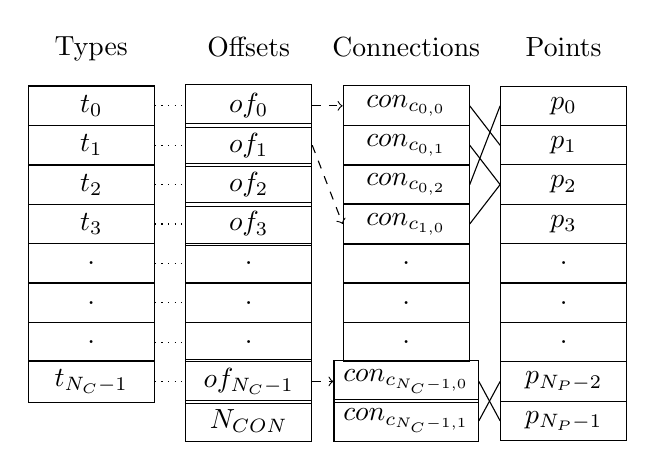
\begin{tikzpicture}
[every node/.style={minimum width=1.6cm, minimum height=0.5cm, anchor=center}]
% Define the array elements
\node[anchor=north] at (0,1) {Types};
\node[draw] (t0) at (0,0) {$t_0$};
\node[draw] (t1) at (0,-0.5) {$t_1$};
\node[draw] (t2) at (0,-1) {$t_2$};
\node[draw] (t3) at (0,-1.5) {$t_3$};
\node[draw] (t4) at (0,-2) {$.$};
\node[draw] (t5) at (0,-2.5) {$.$};
\node[draw] (t6) at (0,-3) {$.$};
\node[draw] (tn_1) at (0,-3.5) {$t_{N_{C}-1}$};

\node[anchor=north] at (2,1) {Offsets};
\node[draw] (of0) at (2,0) {$of_0$};
\node[draw] (of1) at (2,-0.5) {$of_1$};
\node[draw] (of2) at (2,-1) {$of_2$};
\node[draw] (of3) at (2,-1.5) {$of_3$};
\node[draw] (of4) at (2,-2) {$.$};
\node[draw] (of5) at (2,-2.5) {$.$};
\node[draw] (of6) at (2,-3) {$.$};
\node[draw] (ofn_1) at (2,-3.5) {$of_{N_{C}-1}$};
\node[draw] (ofn) at (2,-4) {$N_{CON}$};

\node[anchor=north] at (4,1) {Connections};
\node[draw] (con0_0) at (4,0) {$con_{c_{0,0}}$};
\node[draw] (con0_1) at (4,-0.5) {$con_{c_{0,1}}$};
\node[draw] (con0_2) at (4,-1) {$con_{c_{0,2}}$};
\node[draw] (con1_0) at (4,-1.5) {$con_{c_{1,0}}$};
\node[draw] (cond0) at (4,-2) {$.$};
\node[draw] (cond1) at (4,-2.5) {$.$};
\node[draw] (cond2) at (4,-3) {$.$};
\node[draw] (conn_1_0) at (4,-3.5) {$con_{c_{N_C-1, 0}}$};
\node[draw] (conn_1_1) at (4,-4) {$con_{c_{N_C-1, 1}}$};

\node[anchor=north] at (6,1) {Points};
\node[draw] (p0) at (6,0) {$p_0$};
\node[draw] (p1) at (6,-0.5) {$p_1$};
\node[draw] (p2) at (6,-1) {$p_2$};
\node[draw] (p3) at (6,-1.5) {$p_3$};
\node[draw] (p4) at (6,-2) {$.$};
\node[draw] (p5) at (6,-2.5) {$.$};
\node[draw] (p6) at (6,-3) {$.$};
\node[draw] (pn_2) at (6,-3.5) {$p_{{N_P}-2}$};
\node[draw] (pn_1) at (6,-4) {$p_{{N_P}-1}$};

\draw [dotted] (t0) -- (of0);
\draw [dotted] (t1) -- (of1);
\draw [dotted] (t2) -- (of2);
\draw [dotted] (t3) -- (of3);
\draw [dotted] (t4) -- (of4);
\draw [dotted] (t5) -- (of5);
\draw [dotted] (t6) -- (of6);
\draw [dotted] (tn_1) -- (ofn_1);

\draw [dashed,->] (of0.east) -- (con0_0.west);
\draw [dashed,->] (of1.east) -- (con1_0.west);
\draw [dashed,->] (ofn_1.east) -- (conn_1_0.west);

\draw (con0_0.east) -- (p1.west);
\draw (con0_1.east) -- (p2.west);
\draw (con0_2.east) -- (p0.west);
\draw (con1_0.east) -- (p2.west);
\draw (conn_1_0.east) -- (pn_1.west);
\draw (conn_1_1.east) -- (pn_2.west);
\end{tikzpicture}
\caption{The data structures used to represent an unstructured mesh.}
\label{fig:unstructured-grid}
\end{figure}

The input of a clip algorithm is an unstructured mesh $M$ with scalars $S$ associated with $P$. $S$ can either be a scalar field, such as density, or generated from $P$ using an implicit function $IF(x)$, e.g., a plane, a box, or a sphere. The points $P_{c_i}$ of cell $c_i$ have associated scalar values $S_{c_i}$ of size $N_{P_{c_i}}$.

\begin{figure}[h]
  \centering
  \begin{subfigure}[t]{0.29\linewidth}
    \centering
    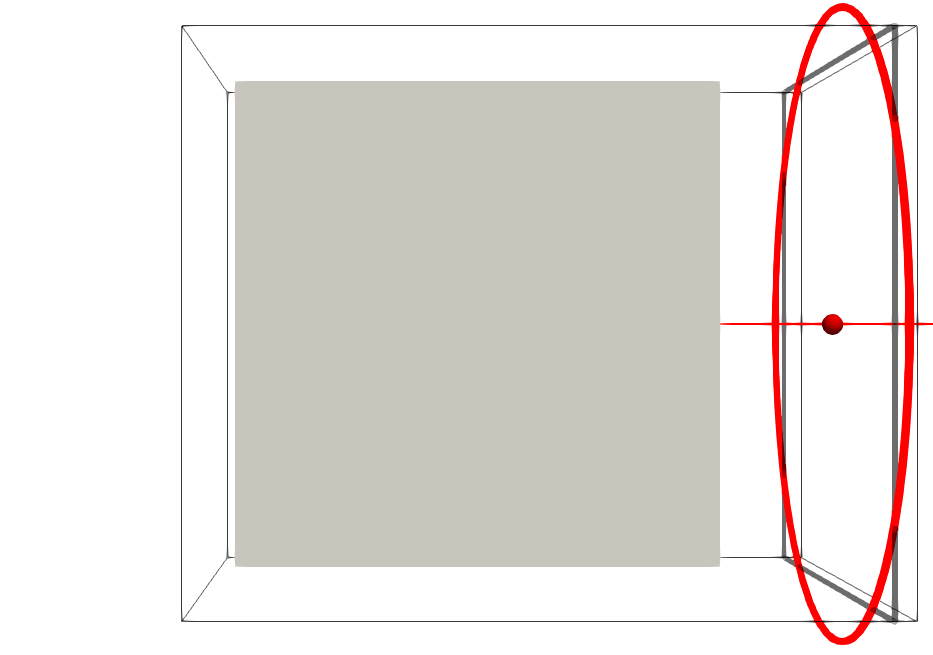
\includegraphics[width=\linewidth]{Figures/Kept-Cell.png}
    \caption{A kept cell.}
    \label{fig:kept-cell}
  \end{subfigure}
  \begin{subfigure}[t]{0.29\linewidth}
    \centering
    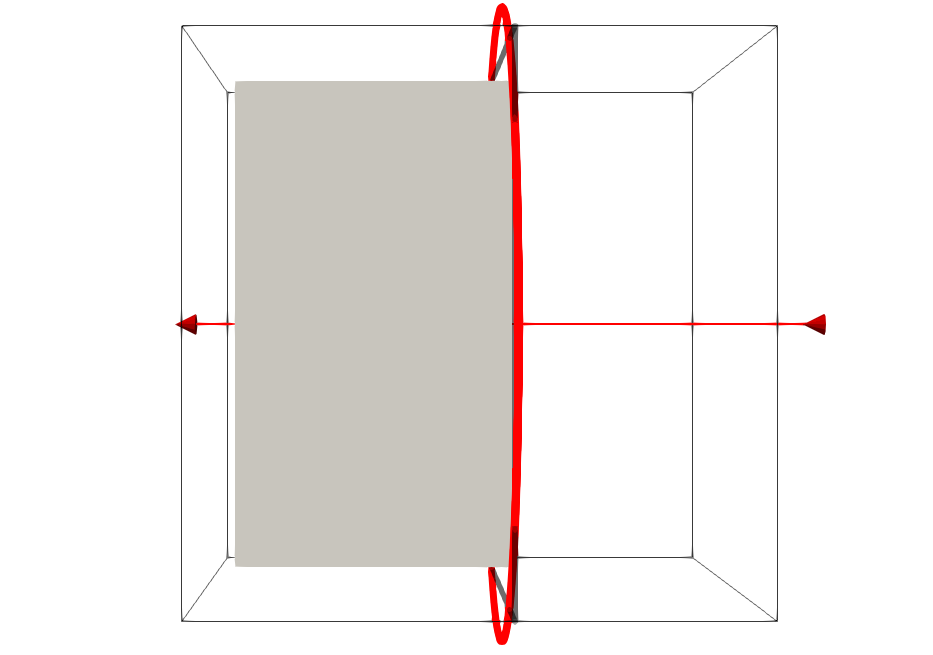
\includegraphics[width=\linewidth]{Figures/Clipped-Cell.png}
    \caption{A clipped cell.}
    \label{fig:clipped-cell}
  \end{subfigure}
  \begin{subfigure}[t]{0.29\linewidth}
    \centering
    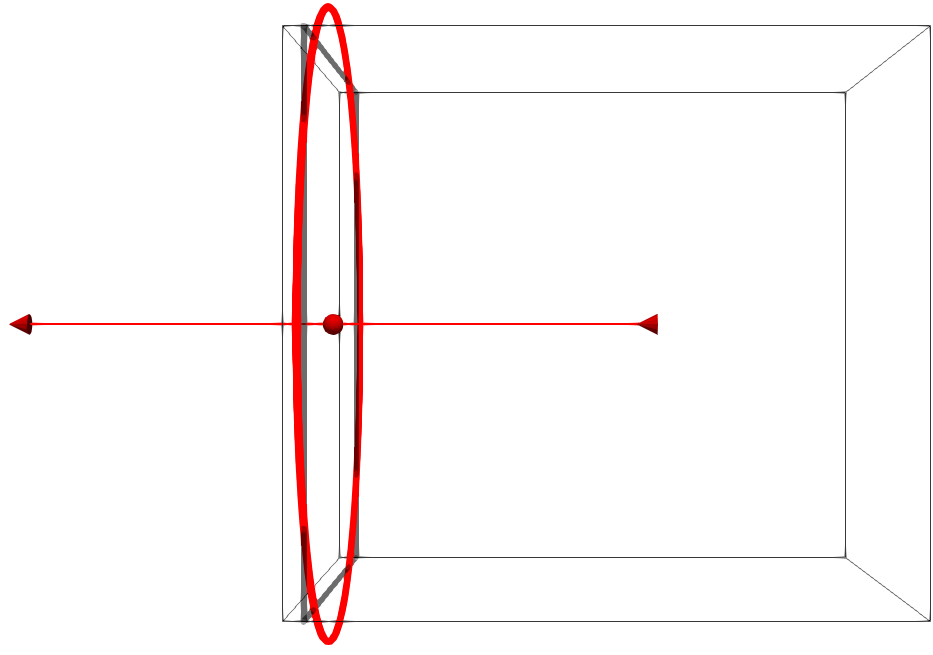
\includegraphics[width=\linewidth]{Figures/Discarded-Cell.png}
    \caption{A discarded cell.}
    \label{fig:discarded-cell}
  \end{subfigure}
  \caption{The three high-level cell cases of a clip algorithm, using a plane implicit function.}
  \label{fig:cell-cases}
\end{figure}

Given an isovalue $v$, a clip algorithm evaluates each cell $c_i$ using its scalars $S_{c_i}$. As shown in Figure \ref{fig:cell-cases}, this evaluation determines if a cell $c_i$ is kept, clipped, or discarded.
$c_i$ is kept if
% $\{\forall s_{c_{i,j}} \in S_{c_i} \mid s_{c_{i,j}} \ge v\}$.
all of $S_{c_i}$ are above $v$.
$c_i$ is discarded if
% $\{\nexists s_{c_{i,j}} \in S_{c_i} \mid s_{c_{i,j}} \ge v\}$.
none of $S_{c_i}$ are above $v$.
$c_i$ is clipped if
% $\{\exists s_{c_{i,j}} \in S_{c_i} \mid s_{c_{i,j}} \ge v\}$.
it is neither kept nor discarded, i.e., some scalars are above $v$ and some are not.

When a cell is kept, its output points mirror its input points. However, when a cell is clipped, new points must be constructed to represent the new geometry. Two types of points may be generated (see Figure \ref{fig:point-types}). Edge points are constructed on an edge of the input mesh and are defined by the two input points of the edge and an interpolation weight. These points, along with points passed directly from the input, are generally shared among multiple output cells. One centroid point, which is defined by input or edge points, may be constructed within the interior of an input cell. Centroid points are exclusive to output cells generated by a specific input cell. They are required, in certain cases, for triangulating the following 3D cell types: voxels, hexahedrons, wedges, and pyramids.

\begin{figure}[h]
    \centering
    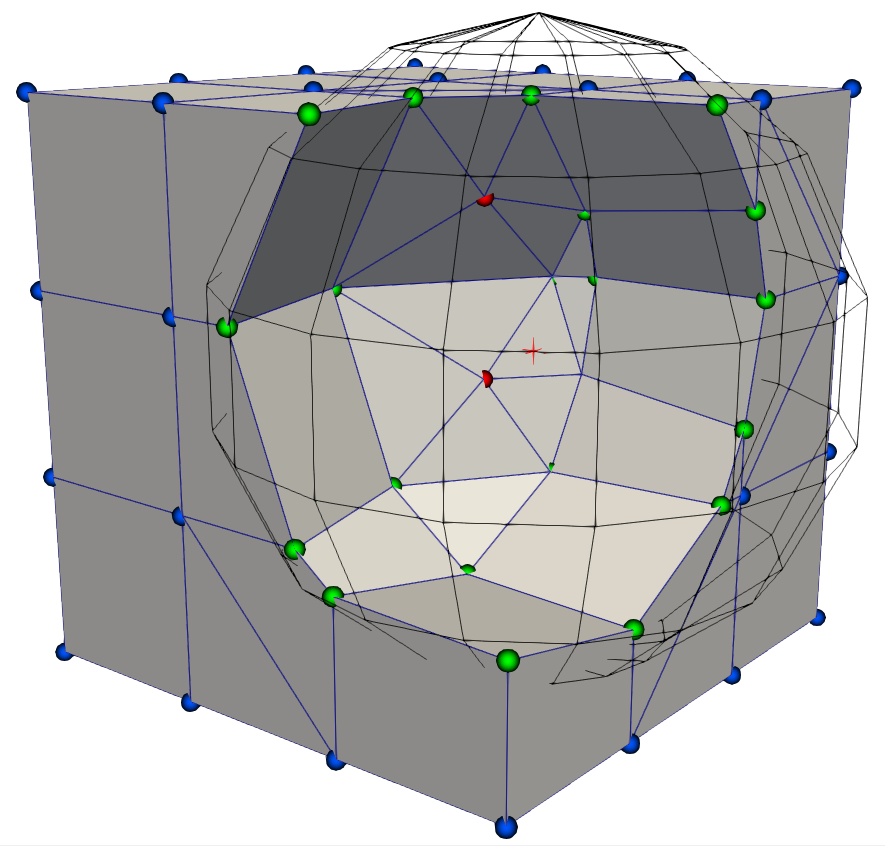
\includegraphics[width=0.555\linewidth]{./Figures/Point-Types.png}
    \caption{Example of the point types that clip algorithms can generate: edge points \textcolor{green}{(green)} and centroid points \textcolor{red}{(red)}.
    Output cells are also constructed from points passed from the input \textcolor{blue}{(blue)}.}
    \label{fig:point-types}
\end{figure}

The output of a clip algorithm is an unstructured mesh $M'$, defined with cells $C'$ and points $P'$ using the same representation demonstrated in Figure \ref{fig:unstructured-grid}. $P'$ incorporates three sets of points: kept points $KP$ which are a subset of $P$, edge points $E$, and centroid points $CEN$ of sizes $N_{KP}$, $N_E$, and $N_{CEN}$, respectively.

\subsection{Algorithmic Constraints, Terminology and Data Structures}
\label{sec:constrains-terminology-data-structures}

The clip algorithms discussed in this paper are designed to process an input mesh $M$ consisting exclusively of first-order cells. These cells adhere to the condition $N_{P_{c_i}}\leq 8$ and belong to one of the following types: vertex, line, triangle, pixel, quadrilateral, tetrahedron, voxel, hexahedron, wedge, and pyramid.

Cells are clipped in much the same way as Marching Cubes \cite{MC} slices cells. A case index array $CI$ of size $N_C$ is constructed by categorizing each cell's incident points as either above or below $v$, and then combining them to form a unique \emph{case index} $ci_i$ for the tessellation. Since only first-order cells with $N_{P_{c_i}}\leq 8$ are supported, the case index $ci_i$ of $c_i$ can be represented by $8$ bits to capture all $2^8$ possible cases, where each bit of $ci_i$ is set as $ci_{i,j} = s_{c_{i,j}} \ge v$.

The case index $ci_i$ of a cell $c_i$ is used to access a clip case table, akin to the Marching Cubes case tables, which facilitate efficient access to information such as the number and types of output shapes, the number of points for each shape, and the types of points within each shape. In this context, shapes encompass both the resulting output cells and optionally a centroid point used to define them.

The computation of kept points $KP$ requires the creation of a point map $M_P$ of size $N_P$. If $m_{p_i} \geq 0$, then $p_i$ is part of $KP$ and $m_{p_i}$ is its point ID in $P'$, else if $m_{p_i} = -1$, then $p_i$ is discarded.  The computation of $E$ uses an edge locator $EL$ that identifies and combines shared edges in adjacent cells. It provides a unique index for an edge's pair of point IDs and stores the linear interpolation weight used to compute coordinates and other fields at this location. The computation of $CEN$ requires the storing of the point IDs defining a centroid point in an input cell.

%%%%%%%%%%%%%%%%%%%%%%%%%%%%%%%%%%%%%%%%%%%%%%%
% Sequential Clip Algorithm
%%%%%%%%%%%%%%%%%%%%%%%%%%%%%%%%%%%%%%%%%%%%%%%
\section{Existing Algorithm: Sequential Clip}
\label{sec:sequential-clip-algorithm}

As described in Section \ref{sec:related-work}, Meredith's clip algorithm comprises four passes. Algorithm \ref{alg:seq-iso} provides a high-level description of its passes.

\begin{algorithm}
% \scriptsize
\caption{Sequential Clip}
\label{alg:seq-iso}
\raggedright
\textbf{Input:} Unstructured mesh $M$ with points $P$, scalars $S$, cells $C$, and isovalue $v$.\\
\textbf{Output:} Clipped unstructured mesh $M'$ with points $P'$ and cells $C'$.
\begin{algorithmic}[1]
    \State \textbf{Pass 1:} Evaluate cells and extract output cells into intermediate type-specific connection arrays with temporary point IDs. Determine number of output cells, edge points, and centroid points.
    \State \textbf{Pass 2:} Define a point map and determine the number of kept points.
    \State \textbf{Pass 3:} Extract kept points, edge points, and centroid points.
    \State \textbf{Pass 4:} Extract the output cells by renumbering the point IDs of the intermediate type-specific connection arrays.
\end{algorithmic}
\end{algorithm}

\subsection{Pass 1: Evaluate Cells}

Initially, the number of kept points $N_{KP}$, edge points $N_E$ and centroid points $N_{CEN}$, is not known. To characterize intermediate output cells' temporary point IDs, three $ID$ segments are defined:  $0 \leq ID < N_P$ (input point), $ID \geq N_P$ (edge point), and $ID < 0$ (centroid point).

In the first pass, the cells are traversed. For each cell $c_i$, its case index $ci_i$ is computed using $S_{c_i}$ to access a case table. Then, the number of output shapes is extracted, and the shapes are traversed.

For each output shape, its points are traversed, and their IDs are defined as follows: If it is an input point, its temporary ID remains the same as its input point. If it is an edge point, it is inserted into the edge locator $EL$; its unique edge ID is retrieved, and the temporary edge point's ID is set as $ID \gets N_{P} + ID$. If it is a centroid point, the temporary centroid point's ID is set as $ID \gets -1 - N_{CEN}$, where $N_{CEN}$ represents the current size of $CEN$.

After defining the point IDs, if the output shape is the special centroid, the centroid is defined using the IDs and incrementally inserted into $CEN$. For other shape types, the cell type is extracted, and the IDs are incrementally inserted into an intermediate type-specific connection array. Finally, upon completion, $N_{C'}$ (including $N_{CON'}$ and $N_{OF'}$), $N_E$, and $N_{CEN}$ become known.

\subsection{Pass 2: Define Point Map}

To compute $KP$, a point map $M_P$ of size $N_P$ is initialized to $-1$, and a $counter \gets 0$ is created. Next, the output point IDs of each cell in the intermediate type-specific connection arrays are traversed. If $0 \leq \textit{ID} < N_P$, and $m_{P_{ID}} = -1$, $m_{P_{ID}} \gets counter$ is set, and the counter is incremented. At the end of this loop, $N_{KP} \gets counter$ and $KP$ is derived
from the non-negative entries in $M_P$.

\subsection{Pass 3: Extract Output Points}

In the third pass, the output points $P'$ are allocated, and the following types of points are inserted: the kept points $KP$, the edge points $E$ that are created using their two point IDs and their linear interpolation weight, and the centroid points $CEN$.

\subsection{Pass 4: Extract Output Cells}

In the fourth pass, the point IDs of each cell in the intermediate type-specific connection arrays are renumbered and written into the output cells $C'$. This renumbering is possible since $N_{KP}$, $N_E$ and $N_{CEN}$ are now known. First, the output cells $C'$ of size $N_{C'}$ are allocated. To populate $C'$, each intermediate type-specific connections array is traversed. For each cell, its type is inserted in $T'$, and its point IDs are renumbered as follows and written in $CON'$ by defining $OF'$:
If $0 \leq ID < N_P$ (input point), then $ID \gets m_{P_{ID}}$.
If $ID \geq N_P$ (edge point), then $ID \gets N_{KP} + ID - N_P$.
If $\textit{ID} < 0 $ (centroid point), then $ID \gets N_{KP} + N_E - ID - 1$.

%%%%%%%%%%%%%%%%%%%%%%%%%%%%%%%%%%%%%%%%%%%%%%%
% Batch-Driven Parallel Clip Algorithm
%%%%%%%%%%%%%%%%%%%%%%%%%%%%%%%%%%%%%%%%%%%%%%%
\section{Proposed Algorithm: Batch-Driven Parallel Clip}
\label{sec:batch-driven-parallel-clip-algorithm}

The proposed batch-driven parallel clip algorithm comprises five passes aimed at enhancing parallel execution and eliminating all deficiencies mentioned in Section \ref{sec:related-work}. Algorithm \ref{alg:par-iso} provides a high-level description of its passes. Subsequent subsections offer comprehensive details on batch definition, detailed descriptions of each pass, and implementation details regarding workload trimming, memory footprint and access, load balancing, and parallel execution.

\begin{algorithm}
% \scriptsize
\caption{Batch-Driven Parallel Clip}
\label{alg:par-iso}
\raggedright
\textbf{Input:} Unstructured mesh $M$ with points $P$, scalars $S$, cells $C$, and isovalue $v$.\\
\textbf{Output:} Clipped unstructured mesh $M'$ with points $P'$ and cells $C'$.
\begin{algorithmic}[1]
    \State \textbf{Pass 1:} Evaluate batches of points and associated scalars against the isovalue, defining a point map, and determining the number of kept points.
    \State \textbf{Pass 2:} Evaluate batches of cells, collect edge points, and determine the number of centroid points, number of output cells, output connections' size, case indices, and batch-related information enabling the writing of cells in Pass 4.
    \State \textbf{Pass 3:} Create the edge locator.
    \State \textbf{Pass 4:} Extract output cells and define the centroid points.
    \State \textbf{Pass 5:} Extract kept points, edge points, and centroid points.
\end{algorithmic}
\end{algorithm}

\subsection{Batch Definition}

Assume a set $A$, such as points or cells, of size $N_A$. $A$ can be partitioned into batches $B_A$ with each batch having a fixed size of $S_B$, except the last batch containing the remainder. Each batch $b_{A_k}$ can have extra variables, such as accumulators, storing statistics related to the algorithm's processing primitive and used for generating output.

Batches can be efficiently removed or trimmed if they meet specific criteria, such as having one of their accumulator variables equal to $0$, thereby enabling workload trimming. The accumulator variables of a batch, which is part of a collection of batches, can be leveraged to calculate global summations. Furthermore, these accumulator variables can be efficiently transformed in-place to offsets using a parallel prefix-sum.

The configurability of the batch size $S_B$, which is evaluated in Section~\ref{sec:batch-size-and-trimming}, 
significantly affects both run-time performance and memory footprint, showcasing noticeable enhancements or deterioration depending on the dataset size.

\subsection{Pass 1: Define Point Map}
\label{sec:par-pass-1}

The batches of points $B_P$ have a size of $N_{B_P}$. Each batch $b_{P_k}$ has an accumulator variable for the number of kept points. Initially, the batches of points are traversed in parallel. For each scalar value $s_i$ of a point $p_i$ in batch $b_{P_k}$, if $s_i \ge v$, then $m_{p_i} \gets 1$, else $m_{p_i} \gets -1$. If $m_{p_i} = 1$, then the accumulator is incremented. Upon completion, the accumulator contains the number of kept points in the batch.

Subsequently, the batches whose accumulator of kept points is zero are trimmed. For the remaining batches, a parallel prefix sum of the accumulated kept points count is computed. The summed values contain the offset in the output points array for the kept points, and the total summation is $N_{KP}$.

Finally, the remaining batches of points are traversed in parallel again. Before traversing each batch $b_{P_k}$, a $counter \gets \text{offset}$ is created. For each $p_i$ in $b_{P_k}$, if $m_{p_i} = 1$, then $m_{p_i} \gets counter$ and the counter is incremented. Eventually, an $M_P$ equivalent to that generated in the sequential algorithm is defined, and $KP$ is determined.

\subsection{Pass 2: Evaluate Cells}

The batches of cells $B_C$ have a size of $N_{B_C}$. Each batch $b_{C_k}$ contains three accumulator variables: output connections' size, number of output cells, and number of centroid points. Initially, the batches of cells are traversed in parallel. For each cell $c_i$ in each batch $b_{C_k}$, its case index $ci_i$ is computed using $S_{c_i}$ to access a case table. Then, the number of output shapes is extracted, and the shapes are traversed.

For each output shape, its points are traversed. Any edge point is inserted into thread-local edge points. Afterwards, if the output shape is the special centroid, the number of centroid points in $b_{C_k}$ is incremented. For other shape types, the number of output cells and their output connections' size in $b_{C_k}$ are incremented.

Once the batch processing is completed, the batches whose number of output cells accumulator is zero are trimmed. Subsequently, the global summation of all accumulators, including $N_{CON'}$, $N_{C'}$, and $N_{CEN}$, is computed, and the accumulators of each batch are converted to offsets. Finally, the thread-local edge points are merged.

\subsection{Pass 3: Create Edge Locator}

The merged edge points undergo parallel sorting, prioritizing the first point's ID and then the second point's ID. This sorting facilitates the identification of duplicate edge points through sequential traversal of the sorted edges, resulting in the formation of the unique edge points $E$ of size $N_E$. The $EL$ is created by defining beginning and ending offsets for each first point ID defining a static hash map. Given the two point IDs defining an edge, $EL$  enables the swift retrieval of a unique edge point ID.

\subsection{Pass 4: Extract Output Cells}

First, output arrays for $CON'$, $OF'$, and $T'$ are allocated using the value of $N_{CON'}$ and $N_{C'}$ computed in Pass 2. Likewise, an array $CEN$ to hold centroid points is allocated using $N_{CEN}$. Then, the trimmed batches of cells are traversed in parallel. For each cell $c_i$ in $b_{C_k}$, its case index $ci_i$ is used to access a case table. Then, the number of output shapes is extracted, and the shapes are traversed.

For each output shape, its points are traversed, and their IDs are defined as follows: if it is an input point, its ID is set as $ID \gets m_{p_{ID}}$; if it is an edge point, its unique ID is retrieved using the edge locator $EL$ and set as $ID \gets N_{KP} + ID$; and if it is a centroid point, its ID is determined using the offset of the number of centroids' accumulator in $b_{C_k}$ and set as $ID \gets N_{KP} + N_E + ID$.

After defining the point IDs, if the output shape is the special centroid, the centroid is defined using the point IDs and is inserted into $CEN$. For other shape types, the cell type is extracted, and point IDs, offset, and cell type are written to $CON'$, $OF'$, and $T'$, respectively, at the correct memory position. This is facilitated by the offsets of the output connections' size and the number of output cells accumulators in $b_{C_k}$, computed at the end of Pass 2. All offsets are then appropriately incremented. Finally, the last offset value is assigned as $of'_{N_{C'}} =N_{CON'}$.

\subsection{Pass 5: Extract Output Points}

As described in Section ~\ref{sec:problem-definition}, there are three types of points: kept points, edge points, and centroid points. With the completion of Pass 4, all necessary information is available to define the output points $P'$. Firstly, the output points $P'$ of size $N_{P'} = N_{KP} + N_E + N_{CEN}$ are allocated. Afterwards, the trimmed batches of input points are traversed in parallel. For each point $p_i$ in $b_{P_k}$, if $m_{p_{i}} > 0$, it is written to $P'$ at position $m_{p_{i}}$. Subsequently, the edges $E$ are traversed in parallel. For each edge $e_i$ with two point IDs and a linear interpolation weight, the edge point is constructed and written to $P'$ at position $N_{KP} + i$. Finally, the centroid points $CEN$ are traversed in parallel. For each centroid $cen_i$, the centroid point is constructed and written to $P'$ at position $N_{KP} + N_E + i$.

\subsection{Workload Trimming}
\label{sec:workload-trimming}

As most cells in a clip operation are either fully kept or entirely discarded, utilizing trimming techniques whenever feasible can significantly reduce the workload. To that end, the following two optimizations are implemented:

\begin{itemize}
    \item \textit{Trim Batches}: In Passes 1, 2, 4, and 5, the algorithm iterates over batches of points or cells. One motivation for this approach is to enable trimming point batches with no kept points in Pass 1 and cell batches that yield no output in Pass 2. As a result, in the second part of Pass 1, in Pass 4, and in Pass 5, fewer batches of points and cells are traversed, respectively, whenever possible.
    \item \textit{Store Case Index}: In Pass 2, we save the 8-bit case index of each cell. Although this requires additional memory, in Pass 4 it enables the quick determination of whether a cell is kept, clipped or discarded without recomputing it by re-accessing the scalars, and therefore, enabling quick cell trimming.
\end{itemize}

\subsection{Memory Footprint and Access}
\label{sec:memory-footprint-and-access}

The clip algorithm is not inherently computationally expensive; therefore, its performance and scalability are constrained by memory bandwidth. It is crucial to minimize memory accesses by reducing the memory footprint and ensuring cache-friendly access or avoiding memory access whenever possible. To achieve this goal, the following five optimizations are implemented:

\begin{itemize}
    \item \textit{Optimize Point Map Computation}: Instead of constructing the point map by traversing the point IDs of output cells to determine if they use an input point, as done in Meredith's and VTK-m's clip algorithms, our proposed algorithm traverses input points. It determines whether they are kept based on their scalar value, as described in Section \ref{sec:par-pass-1}. Traversing the cell connectivity is less cache-friendly because it writes values in the point map in a non-sequential order. Furthermore, points shared by adjacent cells will access the same point map entries multiple times.
    \item \textit{Use 32-bit IDs}: If $N_C \leq 2,147,483,647$, the output cells and point map can be constructed using 32-bit IDs, instead of 64-bit IDs, leading to a halved memory footprint for both.
    \item \textit{Optimize Case Tables}: The case tables used by the sequential clip algorithm, which consist of several arrays per cell type, are packed into one array that can be accessed using an index lookup table. This optimization ensures cache-friendly memory access, especially for input meshes containing more than one cell type. 
    \item \textit{Avoid Accessing Case Tables}: Using the case index, the determination of whether a cell is kept or discarded can be performed without accessing the case tables. Even with the optimized case tables, this improvement proves to be a significant fast-path, since the majority of the input cells are either kept or discarded, and only a small portion is clipped.
    \item \textit{Minimize Accumulators' Memory Footprint}: In contrast to VTK-m's clip algorithm, the batch-driven parallel algorithm allows batches to store accumulators for a sequence of cells, not just one. The higher the batch size, the greater the memory footprint reduction benefit.
\end{itemize}

\subsection{Load Balancing and Parallel Execution}
\label{sec:load-balancing-and-parallel-execution}

Load balancing is challenging when the size of the output cannot be determined \textit{a priori} or when the amount of work differs for ostensibly similar tasks. For all parallel traversals, VTK uses \texttt{vtkSMPTools} to perform parallel execution. \texttt{vtkSMPTools} has four backends: 1) \texttt{Sequential}, 2) \texttt{std::thread} without load balancing, 3) \texttt{OpenMP} using \textit{schedule(runtime)} for load balancing, and 4) \texttt{TBB} \cite{TBB} using $parallel\_for$, which manages a thread pool to process tasks and performs work-stealing when necessary. Based on performance analysis of various algorithms, TBB has been chosen as the default backend for \texttt{vtkSMPTools} due to its load balancing capabilities. Nonetheless, the backend is configurable at runtime using \texttt{vtkSMPTools::SetBackend("BackendName")}.

Alternative approaches to enhance load balancing in parallel isocontouring involve domain decomposition using data structures such as octrees, sphere trees, and contour trees. However, the cost of creating such data structures incurs overhead that is not justifiable for the clip algorithm, as the output size can be orders of magnitude larger compared to isocontouring. In contrast, the batch-driven approach, which includes workload trimming, boosts thread utilization by eliminating batches without work, thereby improving parallel scalability.

The proposed batch-driven parallel clip algorithm has been seamlessly incorporated into VTK and ParaView, both of which possess MPI awareness. Assuming data have already been distributed across MPI nodes, and since no data dependencies exist between nodes, this algorithm can be effortlessly executed at large scales. 

%%%%%%%%%%%%%%%%%%%%%%%%%%%%%%%%%%%%%%%%%%%%%%%
% PERFORMANCE EVALUATION
%%%%%%%%%%%%%%%%%%%%%%%%%%%%%%%%%%%%%%%%%%%%%%%

\begin{figure}[H]
  \centering
  \begin{subfigure}[t]{0.957\linewidth}
    \centering
    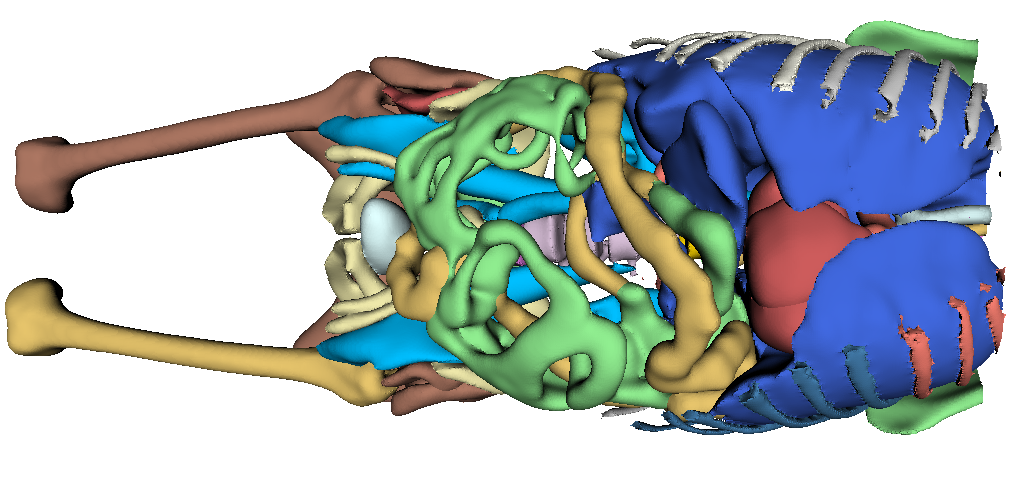
\includegraphics[width=\linewidth]{Figures/Torso.png}
    \caption{A Human Torso generated by parallel Surface Nets \cite{SurfaceNets} using as input an AI-generated segmentation from Total Segmentator \cite{TotalSegmentator}.}
  \end{subfigure}
  \\
  \begin{subfigure}[t]{0.957\linewidth}
    \centering
    \includegraphics[width=\linewidth]{Figures/CX1-car.png}
    \caption{The CX-1 Sedan provided by Altair Engineering, Inc.}
  \end{subfigure}
  \\
  \begin{subfigure}[t]{0.957\linewidth}
    \centering
    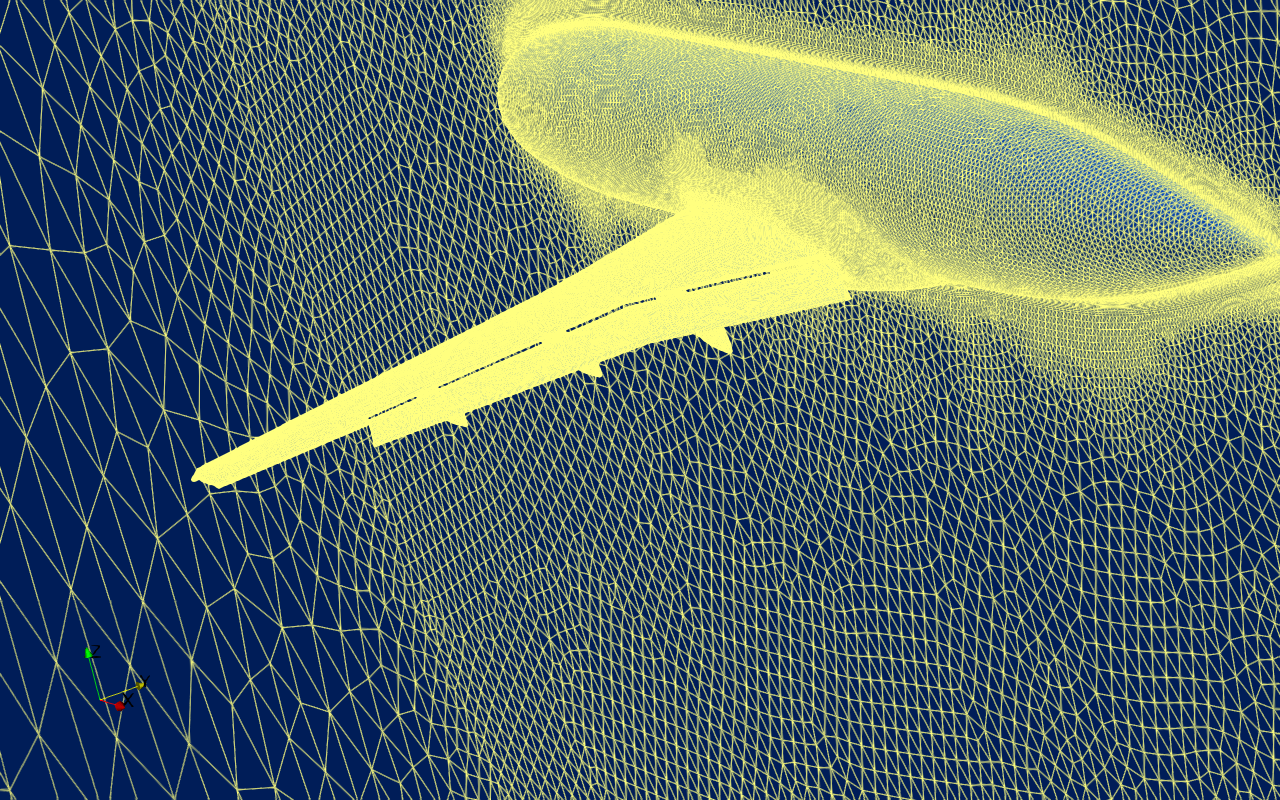
\includegraphics[width=\linewidth]{Figures/JSM.png}
    \caption{The Japan Aerospace Exploration Agency (JAXA) Standard Model (JSM) from the 3rd AIAA CFD High-Lift Prediction Workshop \cite{JAXAModel}.}
  \end{subfigure}
  \\
  \begin{subfigure}[t]{0.957\linewidth}
    \centering
    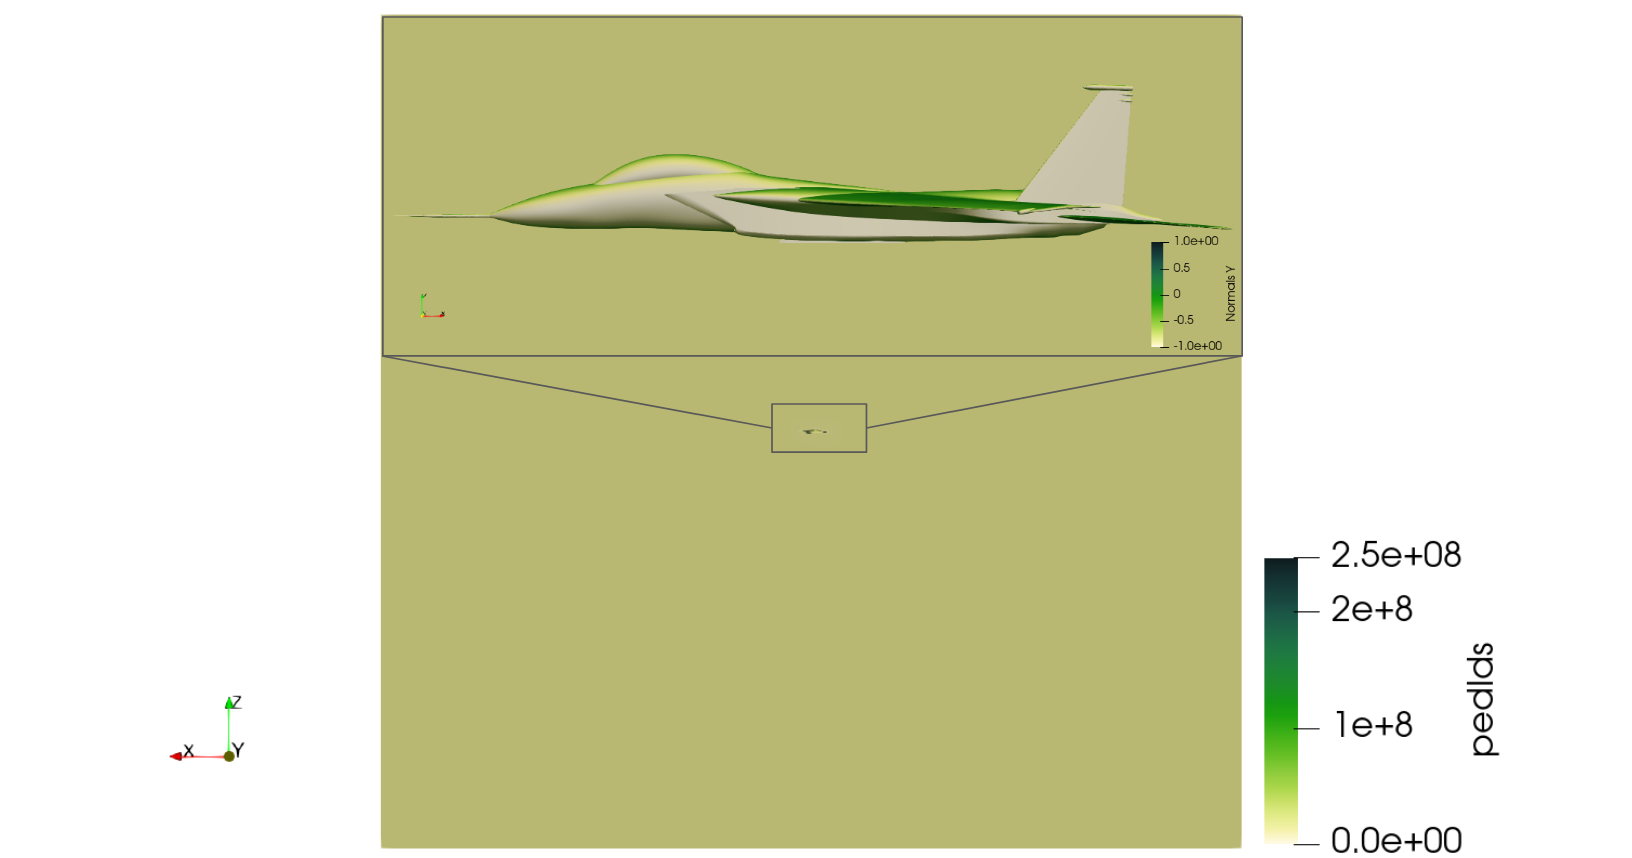
\includegraphics[width=\linewidth]{Figures/F15.png}
    \caption{The fluid volume around an F-15 aircraft, provided by Helden Aerospace, Inc.}
  \end{subfigure}
  \caption{The datasets used for the performance evaluation.}
  \label{fig:datasets}
\end{figure}

\section{Performance Evaluation}
\label{sec:perf-eval}

In this performance evaluation of clip algorithms, we assess the performance of Meredith's sequential algorithm (\textbf{clip-seq}) \cite{Clip}, VTK-m's parallel algorithm (\textbf{clip-m-par}) \cite{VTKm}, and our batch-driven parallel algorithm (\textbf{clip-par}). VTK's first sequential algorithm \cite{VTK} is omitted from this evaluation due to its significant slowness. While all algorithms are MPI-aware thanks to VTK's infrastructure, we opted not to use MPI because an algorithm would simply be executed independently on each node. Thus, analyzing beyond the desktop is unnecessary for the scope of this paper.

The performance evaluation is performed on a computing node that has an Intel Xeon Gold 6226R processor with 16 physical and 32 logical cores (including 16 hyper-threads), and 64GB of DDR4 memory. All algorithms are executed within a Docker container, utilizing the GCC compiler 13.2.0, CMake 3.27.0, and TBB 2021.9 for a standardized evaluation environment  (see Appendix \ref{sec:appendix}).

\subsection{Methods}

We evaluated the clip algorithms' performance using four datasets (see Table~\ref{tab:datasets} and Figure~\ref{fig:datasets}) with varied sizes and cell distributions. For each clip algorithm execution, a dataset is clipped using a plane implicit function with a normal vector $(1, 0, 0)$. Its origin is centered on the dataset's bounds along the y and z axes, while the percentage variable Per controls its position along the x-axis, enabling the creation of output meshes with different sizes. For Per values equal to 20\%, 50\%, and 80\%, we aim to clip most, half, and a small fraction of the dataset, respectively. The run-time and memory footprint are averaged over ten algorithm executions, excluding dataset reading.

\begin{table}[H]
\centering
\caption{Datasets' input size and output size for  $\textit{\{20\%, 50\%, 80\%\}}$ $Per$ values. M stands for millions and K for thousands.}
\label{tab:datasets}
\begin{tabular}{lllrrrr}
\toprule
\multicolumn{3}{c}{Dataset}                            & \multicolumn{1}{c}{Torso} & \multicolumn{1}{c}{CX-1} & \multicolumn{1}{c}{JSM} & \multicolumn{1}{c}{F-15} \\
\midrule
\multicolumn{2}{l}{\multirow{2}{*}{Input}}  &   $N_P$    &  1.4 M  &   8.2 M  &   50.4 M  &  116.4 M  \\
\multicolumn{2}{l}{}                        &   $N_C$    &  2.9 M  &  16.2 M  &  120.0 M  &  246.1 M  \\
\midrule
\multirow{2}{*}{Per} & \multirow{2}{*}{20\%} &  $N_{P'}$  &  0.2 M  &   1.2 M  &    0.9 K  &    3.1 K  \\
                     &                      &  $N_{C'}$  &  0.4 M  &   2.4 M  &    2.0 K  &    9.0 K  \\
\midrule
\multirow{2}{*}{Per} & \multirow{2}{*}{50\%} &  $N_{P'}$  &  0.7 M  &   3.1 M  &   35.3 M  &   91.0 M  \\
                     &                      &  $N_{C'}$  &  1.5 M  &   6.2 M  &   83.0 M  &  192.0 M  \\
\midrule
\multirow{2}{*}{Per} & \multirow{2}{*}{80\%} &  $N_{P'}$  &  1.2 M  &   5.3 M  &   50.4 M  &  116.4 M  \\
                     &                      &  $N_{C'}$  &  2.5 M  &  10.4 M  &  120.0 M  &  246.0 M  \\
\bottomrule
\end{tabular}
\end{table}

\subsection{Batch Trimming and Size}
\label{sec:batch-size-and-trimming}
Figure \ref{fig:batch-trimming} clearly demonstrates the significant impact of trimming on the run-time of the clip-par algorithm across different batch sizes. Notably, the effects of batch trimming are most clearly demonstrated at $Per = 20\%$, highlighting its substantial efficacy. While the median run-time differences with and without trimming are smaller at $Per = 50\%$ and $Per = 80\%$, since they generate more output cells, the reduction in run-time variance is noteworthy. Both aforementioned observations support that batch trimming enhances clip-par's algorithm performance. Therefore, batch trimming is consistently enabled in all subsequent executions.


\begin{figure}[H]
    \centering
    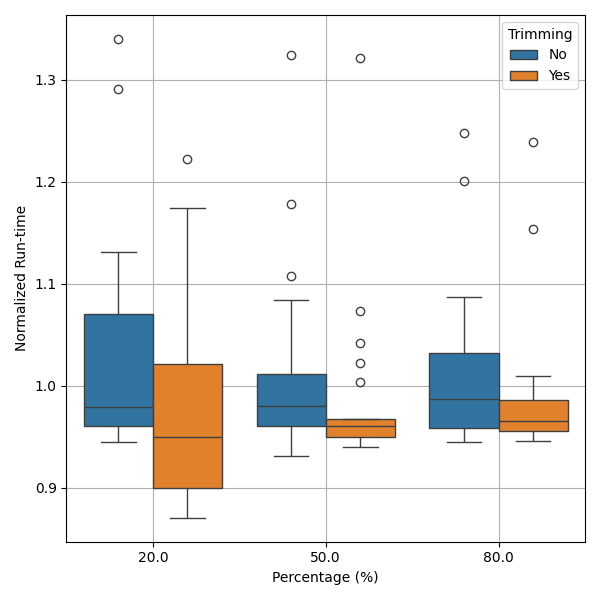
\includegraphics[width=\linewidth]{./Figures/Batch-Trimming.png}
    \caption{Clip-par algorithm's normalized run-time distributions of $\textit{\{20\%, 50\%, 80\%\}}$ $Per$ values with and without batch trimming for varying batches, evaluated using the F-15 dataset, and employing 32 threads. Each run-time is divided by the average run-time with and without trimming for every $Per$ value.}
    \label{fig:batch-trimming}
\end{figure}

\begin{figure}[H]
    \centering
    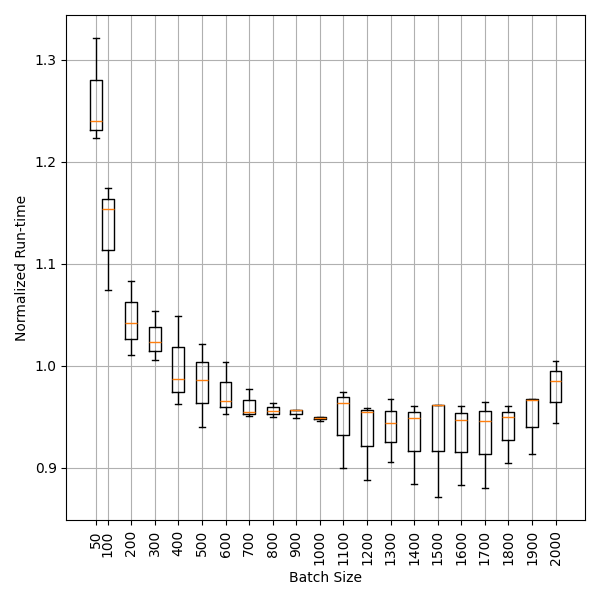
\includegraphics[width=\linewidth]{./Figures/Batch-Size}
    \caption{Clip-par algorithm's normalized run-time distributions of varying batch sizes, with trimming, constructed using the normalized run-times of  $\textit{\{20\%, 50\%, 80\%\}}$ $Per$ values, evaluated using the F-15 dataset, and employing 32 threads. Each run-time is divided by the average run-time with and without trimming for every $Per$ value.
    }
    \label{fig:batch-size}
\end{figure}

Figure \ref{fig:batch-size} clearly demonstrates the significant impact of choosing the appropriate batch size on the run-time of the clip-par algorithm for different $Per$ values with trimming enabled. Notably, very small batch sizes lead to a substantial performance overhead. This stems from the fact that the size of the accumulators increases, and therefore, more memory is accessed to compute the prefix-sums and global summations of the accumulators. When analyzing the ideal batch size, it is evident that the run-times follow a quadratic curve. While several batches with sizes greater than 1000 lead to similar median run-times, the variance of their distribution is larger. Notably, a batch size of 1000 seems to be the optimal point on this curve, demonstrating the least variability across different $Per$ values. Consequently, the optimal batch size of 1000 is chosen and consistently used in all subsequent executions.

\subsection{Run-time Performance}

\begin{table*}[t]
\centering
\caption{
The run-time of clip-seq, clip-m-par, and clip-par algorithms evaluated using the datasets shown in Figure~\ref{fig:datasets} with   $\textit{\{20\%, 50\%, 80\%\}}$ $Per$ values,
and employing 1, 16 and 32 threads ($T$).}
\label{tab:run-time}
\begin{tabular}{lcc@{\quad\quad}rr@{\quad\quad}rr@{\quad\quad}rr@{\quad\quad}rr}
\toprule
\multicolumn{3}{l}{}  & \multicolumn{2}{c}{Torso}  & \multicolumn{2}{c}{CX-1} & \multicolumn{2}{c}{JSM}  & \multicolumn{2}{c}{F-15}     \\
Algorithm  & T  & Per & Time (ms)  & Speed-up      & Time (ms) & Speed-up     & Time (ms) & Speed-up     & Time (ms)    & Speed-up     \\
\midrule
clip-seq   & 1  & 20\% & 142        & 1.00         & 980       & 1.00         & 5,357      & 1.00         & 11,285       & 1.00         \\
clip-m-par & 1  & 20\% & 352        & 0.40         & 2,238     & 0.44         & 14,720     & 0.36         & 30,402       & 0.37         \\
clip-m-par & 16 & 20\% & 82         & 1.73         & 432       & 2.27         & 2,688      & 1.99         & 5,497        & 2.05         \\
clip-m-par & 32 & 20\% & 71         & 2.00         & 414       & 2.37         & 2,369      & 2.26         & 5,010        & 2.25         \\
clip-par   & 1  & 20\% & 100        & 1.42         & 542       & 1.81         & 3,233      & 1.66         & 6,813        & 1.66         \\
clip-par   & 16 & 20\% & 15         & 9.47         & 66        & 14.85        & 389        & 13.77        & 687          & 16.43        \\
clip-par   & 32 & 20\% &\textbf{11} &\textbf{12.91}&\textbf{54}&\textbf{18.15}&\textbf{385}&\textbf{13.91}&\textbf{652}  &\textbf{17.31}\\[1ex]
clip-seq   & 1  & 50\% & 246        & 1.00         & 1,547     & 1.00         & 18,347     & 1.00         & 44,770       & 1.00         \\
clip-m-par & 1  & 50\% & 495        & 0.50         & 3,116     & 0.50         & 30,621     & 0.60         & 81,135       & 0.55         \\
clip-m-par & 16 & 50\% & 109        & 2.26         & 560       & 2.76         & 5,206      & 3.52         & 11,151       & 4.01         \\
clip-m-par & 32 & 50\% & 93         & 2.65         & 513       & 3.02         & 4,641      & 3.95         & 10,081       & 4.44         \\
clip-par   & 1  & 50\% & 132        & 1.86         & 805       & 1.92         & 7,397      & 2.48         & 19,068       & 2.35         \\
clip-par   & 16 & 50\% & 21         & 11.71        & 92        & 16.82        & 888        & 20.66        & 1,854        & 24.15        \\
clip-par   & 32 & 50\% &\textbf{15} &\textbf{16.40}&\textbf{80}&\textbf{19.34}&\textbf{820}&\textbf{22.37}&\textbf{1,497}&\textbf{29.91}\\[1ex]
clip-seq   & 1  & 80\% & 363        & 1.00         & 2,169     & 1.00         & 25,940     & 1.00         & 55,225       & 1.00         \\
clip-m-par & 1  & 80\% & 637        & 0.57         & 3,876     & 0.56         & 40,260     & 0.64         & 93,661       & 0.59         \\
clip-m-par & 16 & 80\% & 124        & 2.93         & 670       & 3.24         & 6,044      & 4.29         & 12,180       & 4.53         \\
clip-m-par & 32 & 80\% & 106        & 3.42         & 600       & 3.62         & 5,412      & 4.79         & 11,210       & 4.93         \\
clip-par   & 1  & 80\% & 172        & 2.11         & 1,116     & 1.94         & 8,307      & 3.12         & 22,508       & 2.45         \\
clip-par   & 16 & 80\% & 24         & 15.13        & 120       & 18.08        & 894        & 29.02        & 2,133        & 25.89        \\
clip-par   & 32 & 80\% &\textbf{20} &\textbf{18.15}&\textbf{95}&\textbf{22.83}&\textbf{884}&\textbf{29.34}&\textbf{1,694}&\textbf{32.60}\\
\bottomrule
\end{tabular}
\end{table*}

Table \ref{tab:run-time} showcases the run-time performance of clip-seq, clip-m-par, and clip-par algorithms. Notably, clip-par stands out with significant speed-ups over clip-seq of up to 3.12x on just 1 thread and up to 32.60x on 32 threads. This enhancement is credited to optimizations detailed in Sections \ref{sec:workload-trimming} and \ref{sec:memory-footprint-and-access} and is underscored by clip-seq's limitations in Section \ref{sec:related-work}. Conversely, clip-m-par shows a noticeable slowdown compared to clip-seq with a single thread, with sub-optimal speed-ups from 0.36x to 0.64x. Despite this, thanks to its parallel capabilities, clip-m-par achieves a noteworthy speed-up of up to 4.93x. The relative slowness of clip-m-par compared to clip-seq with a single thread is attributed to the usage of accumulators per cell. Overall, clip-par is always faster than clip-m-par by up to 7.68x on the same number of threads and faster than clip-seq on a single thread by up to 3.12x.

\begin{figure}[b]
  \centering
  \begin{subfigure}[t]{0.49\linewidth}
    \centering
    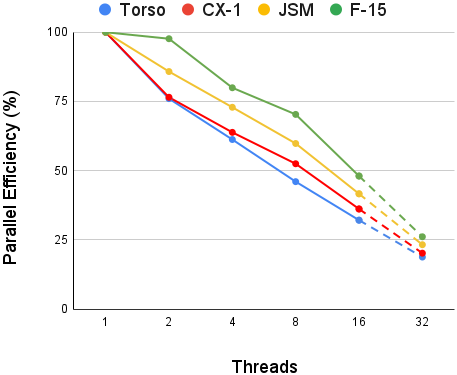
\includegraphics[width=\linewidth]{Figures/Parallel-Efficiency-clip-m-par.png}
    \caption{Clip-m-par's parallel efficiency.}
    \label{fig:par-efficiency-clip-m-par}
  \end{subfigure}
  \begin{subfigure}[t]{0.49\linewidth}
    \centering
    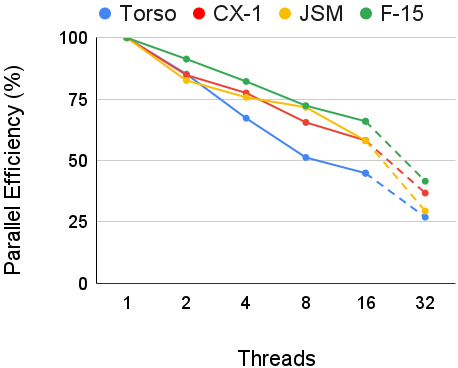
\includegraphics[width=\linewidth]{Figures/Parallel-Efficiency-clip-par.png}
    \caption{Clip-par's parallel efficiency.}
    \label{fig:par-efficiency-clip-par}
   \end{subfigure}
   \caption{The parallel efficiency of the clip-m-par and clip-par algorithms evaluated using the datasets shown in Figure~\ref{fig:datasets} with 80\% $Per$ value, and employing 1, 2, 4, 8, 16 and 32 threads. The dashed lines represent the usage of 16 additional hyper-threads.}
   \label{fig:par-efficiency}
\end{figure}

Overall, as illustrated in Figure \ref{fig:par-efficiency}, it is evident that clip-par demonstrates enhanced parallel efficiency compared to clip-m-par. With 16 and 32 threads, clip-par achieves efficiencies of 66\% and 42\%, respectively. The inability to reach 100\% efficiency is attributed to load balancing challenges, as discussed in Section ~\ref{sec:load-balancing-and-parallel-execution}, and memory bandwidth constraints, as noted in Section \ref{sec:memory-footprint-and-access}. The drop in parallel efficiency from 66\% to 42\% is expected due to the additional 16 threads being hyper-threads. Also, a discernible trend emerges: parallel efficiency declines as the number of threads increases. However, it is important to highlight that parallel efficiency improves with larger datasets.

Table \ref{tab:pass-time} provides a breakdown of the run-time for each pass of the clip-par algorithm. Notable, since $Per$ directly influences the amount of output to extract, and Passes 4 and 5 extract the output, it's understandable that they exhibit high sensitivity to $Per$. Moreover, Pass 3 emerges as the least resource-intensive pass, because $N_E << N_P, N_C$. Lastly, the implicit function computation and Pass 1 demonstrate comparatively lower parallel efficiency.

\begin{table}[h]
\centering
\caption{The run-time of each pass ($P$) of the clip-par algorithm, including the scalar point data computation with the plane implicit function ($IF(x)$),  evaluated using the F-15 dataset with   $\textit{\{20\%, 50\%, 80\%\}}$ $Per$ values, and employing 1 and 32 threads ($T$).}
\label{tab:pass-time}
\begin{tabular}{cc@{\quad}rrrrrr}
\toprule
\multicolumn{2}{l}{} & \multicolumn{6}{c}{Time (ms)}                                                                                                                                        \\
T  & Per & \multicolumn{1}{c}{IF(x)} & \multicolumn{1}{c}{P1} & \multicolumn{1}{c}{P2} & \multicolumn{1}{c}{P3} & \multicolumn{1}{c}{P4} & \multicolumn{1}{c}{P5} \\
\midrule
1  & 20\% & 553   & 276 & 6,178 & 37 & 1      & 1     \\
32 & 20\% & 140   & 38  & 382   & 41 & 1      & 1     \\
1  & 50\% & 549   & 361 & 6,354 & 76 & 9,655  & 1,881 \\
32 & 50\% & 117   & 52  & 400   & 50 & 597    & 171   \\
1  & 80\% & 621   & 383 & 6,104 & 35 & 12,158 & 2,280 \\
32 & 80\% & 116   & 57  & 358   & 42 & 667    & 205   \\
\bottomrule
\end{tabular}
\end{table}

\subsection{Memory Footprint}

Table~\ref{tab:mem-footprint} demonstrates the substantial reduction in memory footprint achieved by the clip-par algorithm, which is up to 4.37 times less than that of clip-seq, thanks to optimizations explained in Section~\ref{sec:memory-footprint-and-access}. In contrast, the memory footprint of clip-m-par exhibits a distinct pattern, increasing by up to one order of magnitude for low $Per$ values and by 1.73x for high $Per$ values compared to clip-seq. In summary, clip-par consistently maintains the smallest memory footprint under most conditions and under the largest memory conditions.

\begin{table}[h]
\centering
\caption{The memory footprint of clip-seq, clip-m-par, and clip-par algorithms evaluated using the datasets shown in Figure~\ref{fig:datasets} with $\textit{\{20\%, 50\%, 80\%\}}$ $Per$ values. The memory footprint is the same regardless of how many threads are being utilized. }
\label{tab:mem-footprint}
\begin{tabular}{lc@{\quad}rrrr}
\toprule
\multicolumn{2}{l}{}                & \multicolumn{4}{c}{Memory (megabytes)}                                                                    \\
\multicolumn{1}{c}{Algorithm} & Per & \multicolumn{1}{c}{Torso} & \multicolumn{1}{c}{CX-1} & \multicolumn{1}{c}{JSM} & \multicolumn{1}{c}{F-15} \\
\midrule
clip-seq   & 20\% & 92        & 581        &\textbf{588}  &\textbf{1,349} \\
clip-m-par & 20\% & 388       & 4,946      & 13,743       & 28,156        \\
clip-par   & 20\% &\textbf{29}&\textbf{230}& 695          & 1,664         \\[1ex]
clip-seq   & 50\% & 196       & 1,058      & 13,375       & 33,294        \\
clip-m-par & 50\% & 447       & 1,925      & 15,991       & 35,914        \\
clip-par   & 50\% &\textbf{53}&\textbf{417}&\textbf{3,295}&\textbf{8,640} \\[1ex]
clip-seq   & 80\% & 302       & 1,592      & 19,008       & 40,370        \\
clip-m-par & 80\% & 523       & 1,969      & 19,715       & 41,788        \\
clip-par   & 80\% &\textbf{80}&\textbf{624}&\textbf{4,348}&\textbf{10,573}\\
\bottomrule
\end{tabular}
\end{table}

% %%%%%%%%%%%%%%%%%%%%%%%%%%%%%%%%%%%%%%%%%%%%%%%
% % CONCLUSIONS AND FUTURE WORK
% %%%%%%%%%%%%%%%%%%%%%%%%%%%%%%%%%%%%%%%%%%%%%%%

\section{Conclusions and Future Work}
\label{sec:conclusions-future-work}

We have designed a batch-driven parallel clip algorithm optimized for clipping unstructured meshes with a continuous point-associated set of scalar data that exhibits high performance and low memory footprint. The inspiration for developing this algorithm comes from the advent of new parallel computing models and the realization that many algorithms need to be redesigned to take full advantage of modern multi-core hardware. Our parallelized clip algorithm operates over fixed-size batches of points and cells. Batches enable rapid workload trimming and parallel processing, leading to a significantly improved run-time performance and memory footprint compared to Meredith's sequential algorithm and VTK-m's parallel algorithm.

In the future, when batch processing capabilities are introduced into VTK-m, we aim to incorporate our proposed batch-driven clipping algorithm, thereby harnessing GPU utilization within the framework. Additionally, our proposed batching technique, along with several concepts from the Flying Edges algorithm, could be potentially used to design an efficient clipping algorithm tailored for structured meshes, such as medical images. Finally, we plan to enhance the parallel Surface Nets discrete isocontouring algorithm \cite{SurfaceNets} by integrating batch processing. We anticipate that this enhancement will substantially improve the processing of segmented medical images that are sparse.

We have adhered to the principles of reproducible science by integrating our batch-driven parallel algorithm into the Open-Source VTK library \cite{VTKBook}. The code has been included in a later version of the \texttt{vtkTableBasedClipDataSet} class. For details regarding the versions of VTK used, please refer to Appendix \ref{sec:appendix}.

% %%%%%%%%%%%%%%%%%%%%%%%%%%%%%%%%%%%%%%%%%%%%%%%
% % ACKNOLEDGEMENTS
% %%%%%%%%%%%%%%%%%%%%%%%%%%%%%%%%%%%%%%%%%%%%%%%

\section{Acknowledgements}
\label{sec:acknowledgements}

The implementation of this work was supported by the Data Analysis and Assessment Center (DAAC) of the United States Department of Defense High-Performance Computing Modernization Program.

This work was also supported in part by the U.S. Department of Energy (DOE) RAPIDS SciDAC project under contract number DE-AC05-00OR22725 and by the Exascale Computing Project (17-SC-20-SC), a collaborative effort of the U.S. Department of Energy Office of Science and the National Nuclear Security Administration.

This paper describes objective technical results and analysis.  Any subjective views or opinions that might be expressed in the paper do not necessarily represent the views of the U.S. Department of Energy or the United States Government.  Portions of this work is funded through a contract with Sandia National Laboratories.  Sandia National Laboratories is a multimission laboratory managed and operated by National Technology \& Engineering Solutions of Sandia, LLC, a wholly owned subsidiary of Honeywell International Inc., for the U.S. Department of Energy’s National Nuclear Security Administration under contract DE-NA0003525.

Special acknowledgments are extended to Altair Engineering, Inc. and Helden Aerospace,  Inc. for their support and provision of datasets used for the performance evaluation of the proposed algorithm. Finally, the authors  would like to express their appreciation for the insightful feedback from  Kevin Garner, Christos Tsolakis, and Cory Quammen during the review  process, which greatly improved the rigor and quality of this research work.

%-------------------------------------------------------------------------
% bibtex
\bibliographystyle{eg-alpha-doi} 
\bibliography{references}       

% biblatex with biber
% \printbibliography                

\pagebreak

\appendix
\section{Reproducibility of Results}
\label{sec:appendix}

To reproduce the results presented in Section \ref{sec:perf-eval}, access the \href{https://github.com/spyridon97/vtk-clip-evaluation}{\textcolor{blue}{vtk-clip-evaluation}} repository. This repository includes the evaluation code along with a link to the used datasets and a Docker image that includes all the built executables used for the performance evaluation. There are six executables: \textit{clip-par-test-various-batchSizes-trimming-no}, \textit{clip-par-test-various-batchSizes-trimming-yes}, \textit{clip-par-pass-time}, \textit{clip-seq}, \textit{clip-m-par}, and \textit{clip-par}. Each executable compiles against a different version of VTK that includes the appropriate version of the \texttt{vtkTableBasedClipDataSet} and \texttt{vtkmClip} classes. The VTK version that is utilized by each executable can be found at its \textit{CMakeLists.txt} in the form of a Git commit SHA.

All executables have the \textit{input filename}, \textit{percentage}, and \textit{number of iterations} parameters, while the parallel ones also have the \textit{number of threads} parameter. At the end of each execution, the following information is printed: the memory used by the dataset in kilobytes, the average time spent by each algorithm in milliseconds, and the maximum memory used by the executable in kilobytes. The memory footprint of the algorithm is determined by subtracting the memory used by the dataset from the maximum memory used by the executable. The following command shows an output example of the clip-par executable.

\lstdefinelanguage{BashOutput}{
  basicstyle=\ttfamily\color{black},
  moredelim=**[is][\color{blue}]{|}{|},
  moredelim=**[is][\color{red}]{~}{~}
}

\begin{lstlisting}[language=BashOutput]
$ /usr/bin/time -vv\
      ./clip-par ./Torso.vtu 0.5 1 8
Origin: 490.803, 287.599, 648.45
Normal: 1, 0, 0
Number of input cells: 2867390
Number of input points: 1404982
~Memory used by dataset in KB: 139372~
Number of output cells: 1454024
Number of output points: 720730
~Time in ms: 19~
Command being timed:\
      "./clip-par ./Torso.vtu 0.5 1 8"
...
~Maximum resident set size (kbytes): 197924~
...
\end{lstlisting}

\end{document}


